\documentclass[a4paper,12pt]{article}

% Packages
\usepackage[utf8]{inputenc}
\usepackage{geometry}
\usepackage{titlesec}
\usepackage{lipsum} % for generating dummy text
\usepackage{graphicx}
\usepackage{caption}
\usepackage{subcaption}
\usepackage{listings}
\usepackage{amsmath}
\usepackage{amssymb}                                                                                                                                                            
\usepackage{xcolor}
\usepackage{circuitikz}

% Page setup
\geometry{a4paper, margin=1in}
\setlength{\parindent}{0pt}
\setlength{\parskip}{5pt}

% Title setup
\title{\textbf{Electrical Machines} \\
        \vspace*{0.3em}
        \large{Assignment 2} }                                              
\author{Ajay Krishnan K \\  EE22BTECH11003}
\date{February 24, 2024}

% Section and subsection formatting
\titleformat{\section}[block]{\normalfont\Large\bfseries}{\thesection}{1em}{}
\titleformat{\subsection}[block]{\normalfont\large\bfseries}{\thesubsection}{1em}{}
\titleformat{\subsubsection}[block]{\normalfont\normalsize\bfseries}{\thesubsubsection}{1em}{}

% Code listing settings
\lstdefinestyle{mystyle}{
    language=Matlab,
    basicstyle=\ttfamily\small,
    breaklines=true,
    keywordstyle=\color{blue},
    commentstyle=\color{green!40!black},
    stringstyle=\color{red},
    % numbers=left,
    % numberstyle=\tiny,
    frame=single,
    showspaces=false,
    showstringspaces=false,
}

\lstset{style=mystyle}

\begin{document}
\maketitle

\section*{Problem}
Simulate DC shunt machine using dynamic equations and plot the variations for the following quantities:
\begin{enumerate}
    \item Supply voltage
    \item Load current
    \item Field current
    \item Speed
\end{enumerate}

\section*{Solution}
The dynamic equations for a DC shunt machine are given by:
\begin{align*}
    V   & = E + I_a R_a + L_a\frac{dI_a}{dt} \\
    E  & = K_m \omega                   \\
    T_m & = K_m \Phi I_a                   \\
    T_f & = J \frac{d\omega}{dt} + B\omega
\end{align*}

Where:
\begin{align*}
    V      & = \text{Supply voltage}          \\
    E      & = \text{Back emf}                \\
    I_a    & = \text{Armature current}        \\
    R_a    & = \text{Armature resistance}     \\
    R_f    & = \text{Shunt field resistance}  \\
    L_a    & = \text{Armature inductance}     \\
    T_m    & = \text{Mechanical torque}       \\
    T_f    & = \text{Friction torque}  \\
    K_m    & = \text{Machine constant}        \\
    \Phi   & = \text{Flux}                    \\
    % K      & = \text{Back emf constant}       \\
    \omega & = \text{Speed}                   \\
    J      & = \text{Moment of inertia}       \\
    B      & = \text{Coefficient of friction}
\end{align*}

The equivalent circuit of a DC shunt machine is shown below.
\begin{figure}[h!]
    \centering
    \includegraphics*[scale=0.5]{./figs/circuit.png}
    \caption{Equivalent circuit of a DC shunt machine}
    \label{fig:dc_shunt_machine}
\end{figure}

The above equations can be solved using numerical methods. The following code simulates the DC shunt machine and plots the variations of the quantities mentioned in the problem statement.

\newpage

\lstinputlisting[language=Matlab]{code/em.m}

The above code simulates the DC shunt machine and plots the variations of the quantities mentioned in the problem statement. The following plots show the variations of the quantities over time.

\begin{figure}[h]
\centering
\begin{subfigure}{0.45\textwidth}
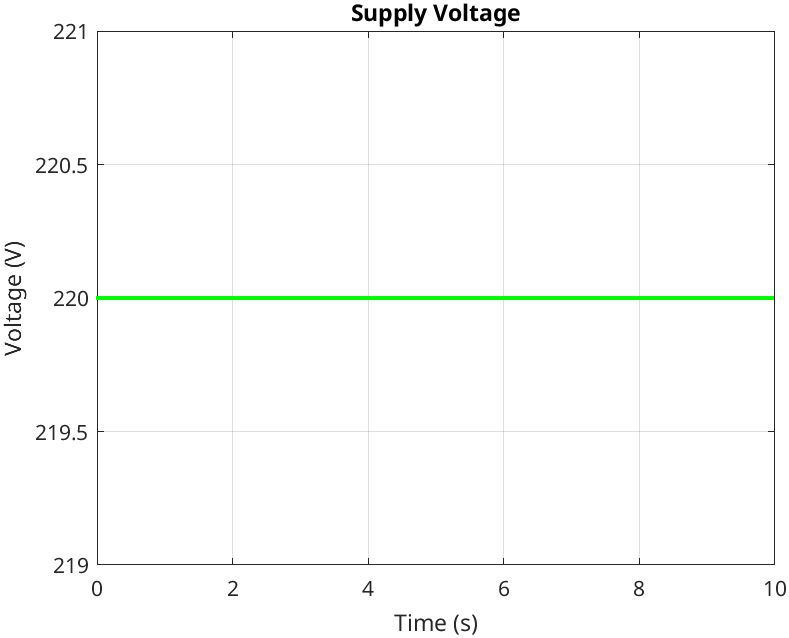
\includegraphics[width=\textwidth]{code/supl.png}
\caption{Supply voltage}
\end{subfigure}
\begin{subfigure}{0.45\textwidth}
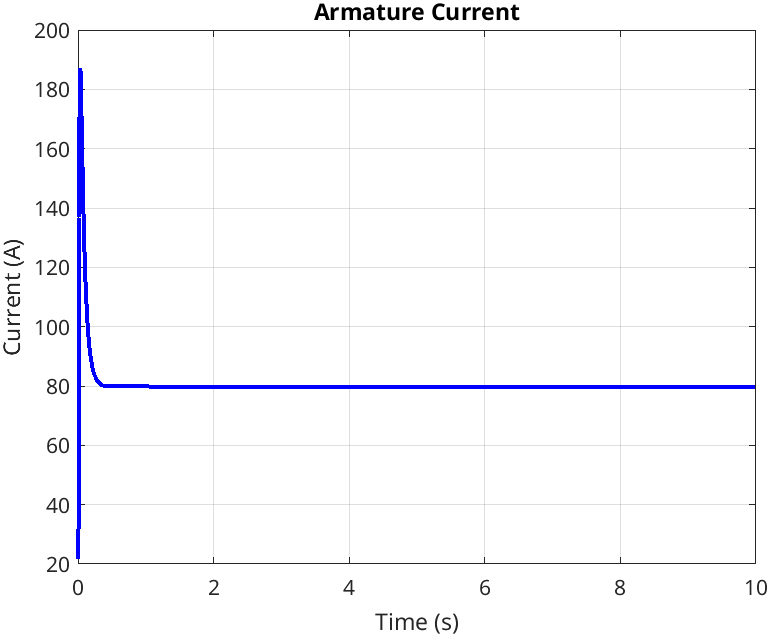
\includegraphics[width=\textwidth]{code/Ia.png}
\caption{Load current}
\end{subfigure}
\begin{subfigure}{0.45\textwidth}
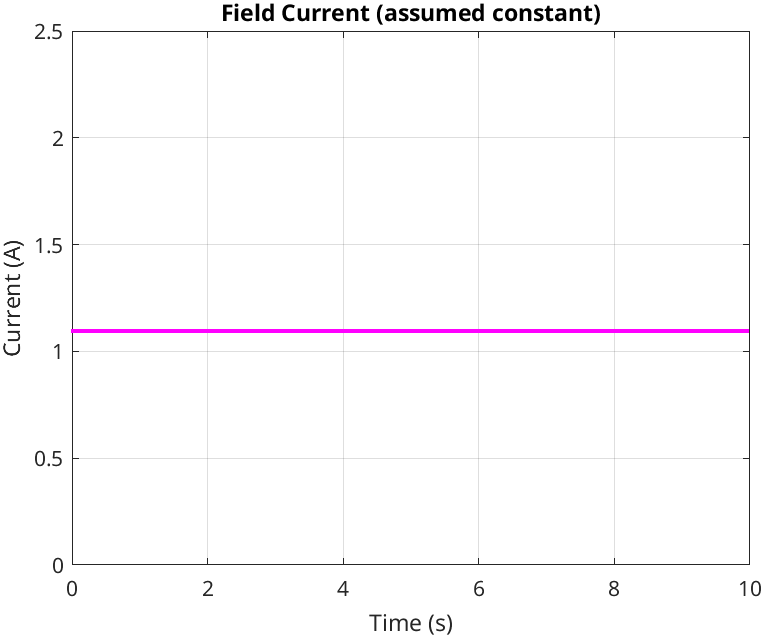
\includegraphics[width=\textwidth]{code/if.png}
\caption{Field current}
\end{subfigure}
\begin{subfigure}{0.45\textwidth}
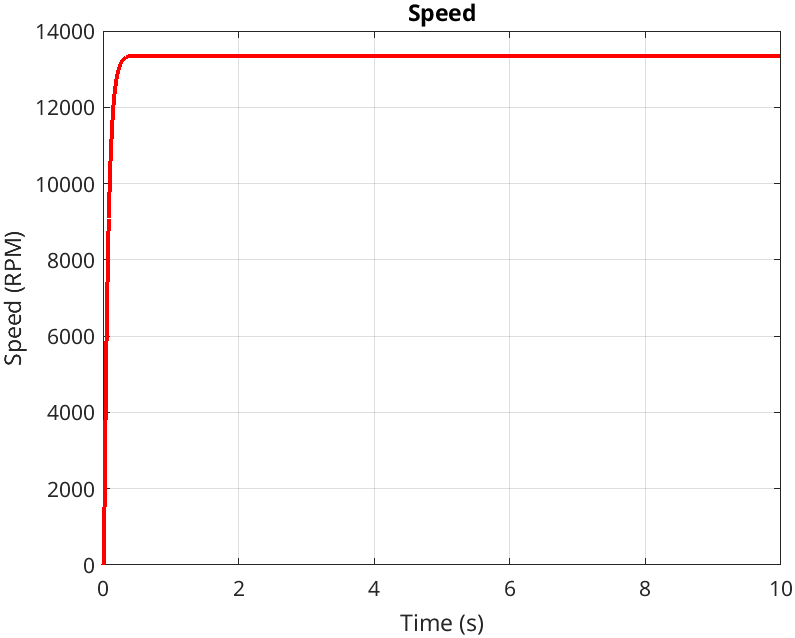
\includegraphics[width=\textwidth]{code/Speed.png}
\caption{Speed}
\end{subfigure}
\end{figure}
\end{document}